A sparse grid that is fully nested and well suited for local adaptivity, which
we required previous, can be constructed using the (one-dimensional)
Newton--Cotes rule \cite{klimke2006, ma2009}. For each level, the rule is merely
a set of equidistant nodes on an interval, which is $[0, 1]$ in our case.

\begin{remark}
Equidistant nodes are known to perform purely when the interpolating functions
are chosen to be polynomials (Runge's phenomenon). However, it is not a concern
for us as our basis functions are not exposed to this problem.
\end{remark}

The rule comes in two flavors: closed and open. The only difference between the
two is that the former includes the endpoints, that is, 0 and 1, while the
latter does not. Now, at the end of \sref{smolyak-algorithm}, we postulated that
the assumption in \eref{tensor-exactness} was needed to proceed. The closed rule
satisfies this assumption while the open one violates it close to the boundaries
of the interval. However, according to our numerical experiments and as noted in
\cite{klimke2006}, the open Newton--Cotes rule is a viable option as it performs
well in practice.

Despite the minor concern noted above, we have opted to present the open
Newton--Cotes rule in the paper as it is a better match for the transformation
in \eref{transformation}. The problem with 0 and 1 is rather technical and is as
follows. The inverse of the Gaussian distribution function, $\Phi^{-1}$, maps 0
and 1 to $-\infty$ and $+\infty$, respectively; as shown in
\eref{transformation}, the resulting vector then gets multiplied by a matrix.
Since certain algebraic operations with infinite values are undefined---for
instance, $0.42 \times (+\infty) + 0.27 \times (-\infty)$---this particular
transformation in \eref{transformation} might pose implementation difficulties,
which we would like to avoid by choosing a rule without the endpoints.

\begin{figure}[t]
  \centering
  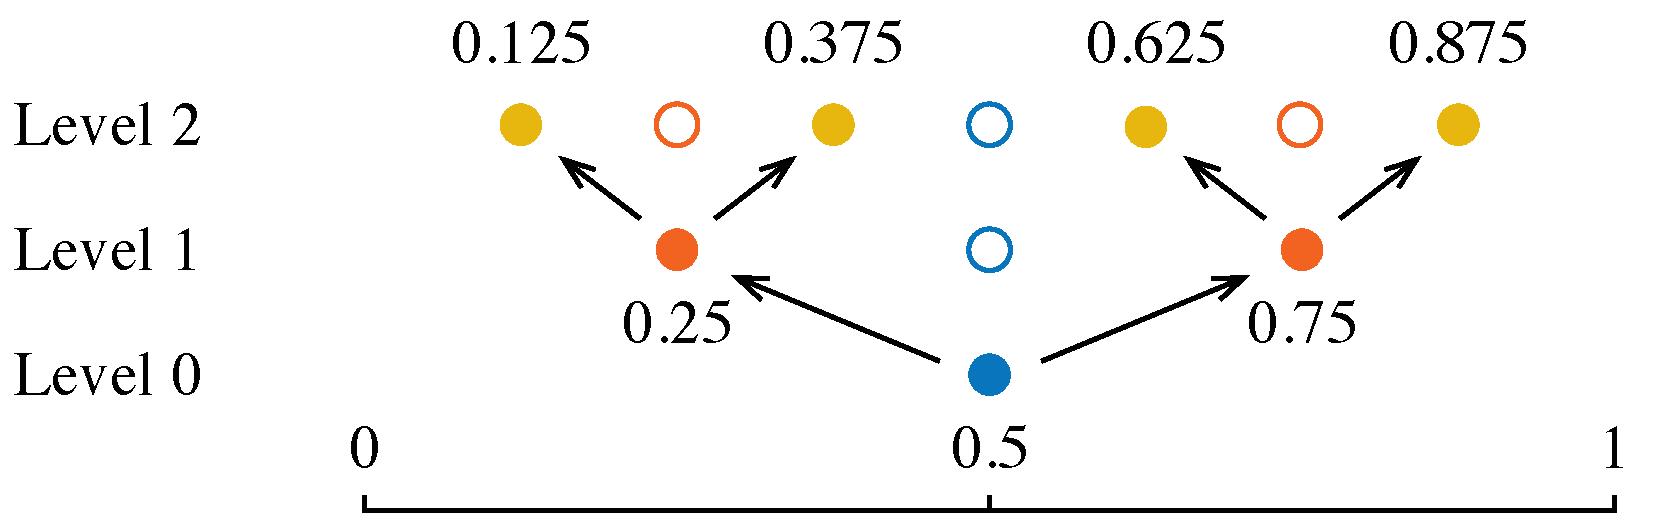
\includegraphics[width=1.0\columnwidth]{include/assets/figures/rule.pdf}
  \caption{
    An illustration of the open Newton--Cotes rule. On each level, the dots
    correspond to the nodes introduced by that particular level, and the wholes
    correspond to the nodes inherited from the previous levels.
  }
  \flab{rule}
\end{figure}

The open Newton--Cotes rule of level $i \in \natural$ is
\[
  \X^i = \left\{ x^i_j = \frac{j + 1}{\n_i + 1}: j \in \index(i) \right\}
\]
where $\index(i) = \left\{ 0, \dots, \n_i - 1 \right\}$ with $\n_i = 2^{i + 1} -
1$. The first three levels of the rule are depicted in \fref{rule}. It can be
seen that the number of nodes (in one dimension) grows as 1, 3, 7, 15, 31, and
so on, and the rule is fully nested. In multiple dimensions, the nodes are
formed as shown in \eref{collocation-nodes}.

\fref{rule} also illustrates the refinement strategies suitable for this grid.
The arrows emerging from a node connect the node with its next-level neighbors.
The number of such neighbors is two in one dimension and $2 \nin$ in general.
Formally, for a pair $(\vi, \vj)$, the neighbor pairs are
\[
  \left\{ \Big( (i_1, \dots, i_k + 1, \dots, i_\nin), (j_1, \dots, 2 j_k + c, \dots j_\nin) \Big) \right\}_{k, c}
\]
for $k = 1, \dots, \nin$ and $c \in \{ 0, 2 \}$. Whenever a node is to be
refined, some or all of its neighbors can be chosen for function evaluation. The
simplest strategy is to include all $2 \nin$ neighbors, which is what we shall
do.
